\chapter{Les processus}
\begin{multicols}{2}
\section{Introduction}

Les systèmes d'exploitation modernes sont tous capables de faire
exécuter plusieurs tâches en même temps.  Sous Unix, la commande
\texttt{top} vous permet de voir les tâches en cours : sur un
ordinateur personnel vous constaterez qu'il en a au moins une bonne
centaine, plusieurs milliers sur un serveur.

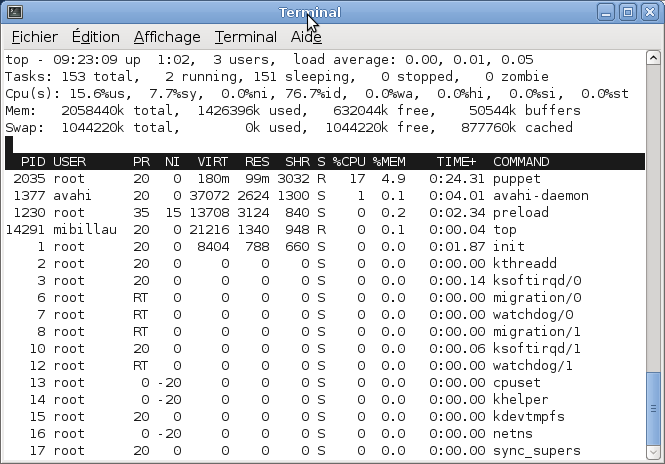
\includegraphics[width=\linewidth]{memoire-images/top.png} 

Mais matériellement, un processeur ne peut exécuter qu'une instruction
à la fois. Même si les ordinateurs possèdent plusieurs processeurs, on
est loin du compte : il n'y a pas un processeur par
programme.\footnote{Dans la suite du cours, pour simplifier, on
  considère des machines à un seul processeur. Avec plusieurs processeurs,
il y a des complications intéressantes, mais les principes de bas sont les mêmes.}


Le déroulement parallèle de ces tâches est donc une \emph{illusion} : en
réalité le processeur consacre un peu de temps ``faire avancer'' une
tâche, puis passe à une autre etc. à tour de rôle.  C'est la rapidité
de cette alternance, quelques millisecondes par tâche, qui donne
l'impression, à notre échelle, que tout avance en même temps.

Une des fonctions importantes d'un système multitâche est donc de gérer les \emph{commutations de contexte} : il doit 
\begin{itemize}
\item noter l'état de la tâche en cours (sauvegarde du contexte)
\item choisir une des tâches (\texttt{ordonnancement})
\item la relancer dans l'état où elle était arrêtée (restauration du contexte)
\end{itemize}

\section{Histoire}

\subsection{Multitâche}
Les systèmes d'exploitation multi-tâches sont apparus très rapidement dans
l'histoire de l'informatique.

\begin{itemize}
\item Ordinateur Gamma 60 de la société Bull, en 1958 \url{http://fr.wikipedia.org/wiki/Gamma_60}. 
%Le premier exemplaire a été livré à la SNCF. 
%Avec  ses 6 imprimantes et  16 dérouleurs de bande, il occupait 360 $m^2$.

%\begin{center}
%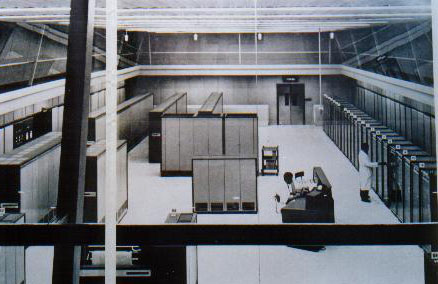
\includegraphics[width=\linewidth]{Historique/Gama2_60.jpg} \\
%source : \url{http://histoireinform.com/Histoire/+infos2/chr4infa.htm}
%\end{center}


\item Ordinateur LEO III de la société Lyons, 1961.

\begin{center}
% http://www.ampneycrucis.f9.co.uk/PARK/1Leo3Operating.jpg
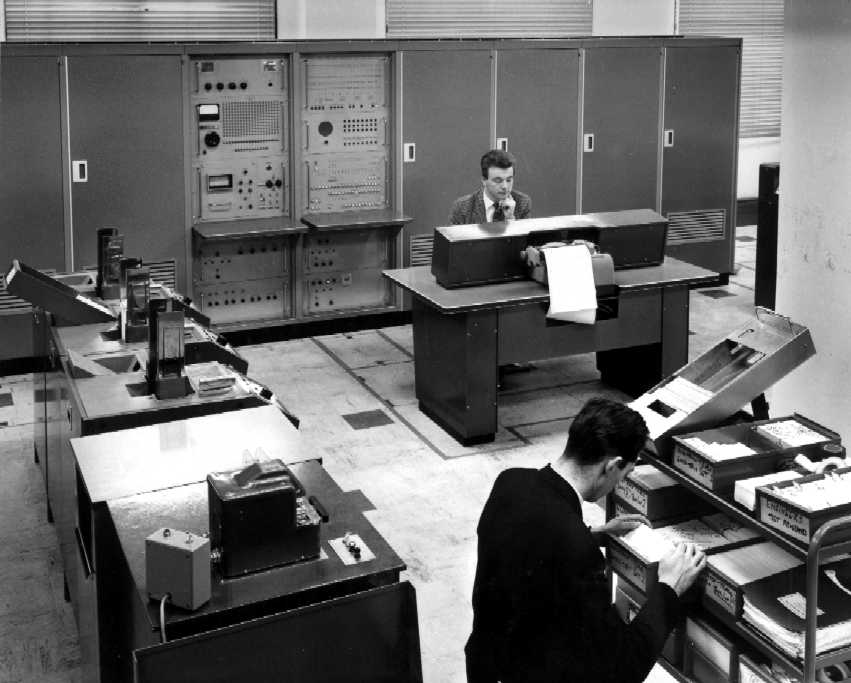
\includegraphics[width=\linewidth]{Historique/1Leo3Operating.jpg} \\
\end{center}

La société Lyons regroupait une chaîne de
restaurants, des hôtels et des activités dans l'alimentaire
(biscuits). Grande utilisatrice de machines à cartes perforées pour sa gestion, elle a
compris avant beaucoup d'autres l'intérêt des recherches qui étaient
menées sur les calculateurs électroniques (EDSAC, à Cambridge). Elle a
donc embauché un technicien radar, loin de son coeur de métier, 
\footnote{Ce n'est pas un cas isolé : Honeywell (spécialiste de la
  régulation de chauffage) et Boeing (avions) ont aussi fabriqué des
  ordinateurs. Et plus tard le premier micro-ordinateur a été fabriqué
  en France pour l'INRA (Institut National de Recherche Agronomique),
  le Micral en 1972.}  pour développer ses propres ordinateurs pour
ses applications de gestion. Le LEO~I (Lyons Electronic Office) est sorti en
1951, et d'autres modèles ont suivi qui ont été commercialisés hors de la société Lyons.
\footnote{
Sur le site \url{http://www.leo-computers.org.uk/} des anciens
employés de LEO Computers, vous trouverez de nombreuses photos
et descriptions (et même des enregistrements de l'ambiance des salles machine).
}
\end{itemize}

\paragraph{L'objectif} du multi-tâches est évident :  si plusieurs 
programmes s'exécutent en même temps, ils utilisent les divers
périphériques en parallèle, ce qui rentabilise au mieux l'installation
informatique : on augmente le nombre de programmes que l'on peut faire
exécuter dans une journée d'utilisation.

\end{multicols}
\subsection{Exemple : intérêt du multi-tâches}

Imaginons deux tâches A et B: 
\begin{itemize}
\item le chargement de A  depuis le lecteur de cartes dure 20 secondes, elle fait du calcul pendant 30 secondes, et l'impression des
résultats prend 1 minute ;
\item le chargement de la seconde B dure  10 secondes, son calcul 20 secondes et l'impression 30 secondes.
\end{itemize}

\begin{multicols}{2}

Le graphique ci-contre montre ce qui se passe sous le contrôle d'un ``moniteur
d'enchaînement de travaux''. La tâche B n'est chargée en mémoire que
quand A s'est terminée ($t=110 s$) et se termine à $t=170 s$.

Le processeur a travaillé $30 + 20 = 50s$, soit un taux d'occupation de 
$50/170 = 29,4 \%$.
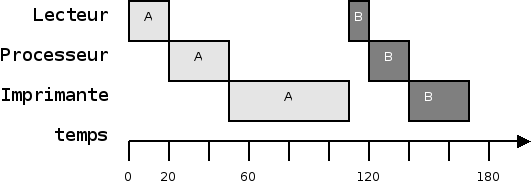
\includegraphics[width=.95\linewidth]{memoire-images/exemple-multitache-1.png}

\end{multicols}
\begin{exercice}
\begin{itemize}
\item calculez le taux d'occupation du lecteur de cartes
\item calculez le taux d'occupation de l'imprimante.
\end{itemize}
\end{exercice}

\begin{multicols}{2}
Voici maintenant le déroulement dans un système multi-tâches ; la tâche B est
chargée dès que le lecteur a été libéré, puis est exécutée quand le processeur
est libre, etc.
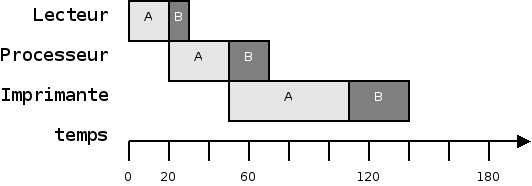
\includegraphics[width=.95\linewidth]{memoire-images/exemple-multitache-2.png}
\end{multicols}

\begin{exercice}
\begin{itemize}
\item Calculez les taux d'occupation, comparez avec les chiffres précédents.
\item Même question si on commence par exécuter B au lieu de A.
\item Imaginons qu'il s'y ajoute une troisième tâche C semblable à B. Représentez le déroulement dans les deux cas (enchaînement séquentiel et multi-tâches). Comparez les chiffres.
\end{itemize}
\end{exercice}

\subsection{Du \emph{batch} au \emph{time sharing}}


\paragraph{Traitement conversationnel.}  Un
nouveau besoin apparaît à la fin des années 50 : avec l'utilisation de
terminaux interactifs : telex transformés, machines à écrire
électriques, et écrans alphanumériques.  Chaque utilisateur doit avoir
l'impression d'utiliser une machine ``réactive'' : si un collègue
lance un programme de calcul lourd (quelques milliers de décimales de
$\pi$)\footnote{ou un programme qui boucle, comme ça arrive parfois.},
cela ne doit pas empêcher les autres de travailler en monopolisant
complètement le temps du processeur.


C'est la prise en compte de cette contrainte qui conduit au \emph{time
  sharing} : le temps du processeur doit être partagé ``équitablement''
entre les utilisateurs.


\begin{multicols}{2}
\subsection{Support matériel du multi-tâches : les interruptions}

Pour être réalisé, le multi-tâche nécessite l'ajout
de quelques quelques fonctionnalités techniques sur le matériel.

En particulier, il ne serait pas raisonnable de devoir interroger
constamment les périphériques pour savoir si les opérations qu'on leur
a confiées (et qui sont attendues par certaines tâches) sont terminées
ou non. Cette \emph{boucle d'attente active} consommerait beaucoup de
temps du processeur, temps que l'on souhaite consacrer à l'exécution de
programmes ``utiles''.

L'ordinateur comporte donc des circuits spécialisés (contrôleurs de
périphériques, en terminologie moderne) à qui le processeur confie
l'exécution des entrées-sorties. Quand l'opération est terminée, le
contrôleur envoie une \texttt{interruption}, signal électrique qui
provoque le déroutement vers une ``routine de traitement de
l'interruption'' située à une adresse convenue.

\paragraph{Dans un ordinateur multi-tâches,}  les interruptions ``réveillent'' le
système d'exploitation, qui peut alors débloquer les tâches qui
attendaient la fin de ces opérations.

D'autres mécanismes matériels sont également nécessaires pour la
multiprogrammation, en particulier il faut \emph{protéger l'espace mémoire
de chaque tâche}, pour éviter qu'une autre tâche y accède indûment.
La gestion de la mémoire fait l'objet d'un autre chapitre.

\subsection{Support logiciel}

Avant la multiprogrammation, les systèmes d'exploitation étaient des
\emph{moniteurs d'enchaînement de travaux} assez très rudimentaires
chargés au début de la mémoire au démarrage de la machine, et dont le
rôle était simplement : 
\begin{enumerate}
\item de lire un programme exécutable (par exemple sur une bande magnétique) et de le copier
un peu plus loin en mémoire,
\item de lancer son exécution,
\item et passer au suivant quand le programme s'est achevé.
\end{enumerate}

Avec plusieurs tâches présentes simultanément, le système
d'exploitation devient plus complexe : il doit traiter les
interruptions provenant des périphériques, faire les commutations de
contexte, gérer le partage de la mémoire, etc.



 
\section{Définitions}
\subsection{Les processus}

Le \textbf{processus} est une entité abstraite qui sert à représenter
    un \textbf{programme en cours d'exécution}.

Un processus regroupe :
    \begin{itemize}
      \item le \textbf{code} du programme : un espace mémoire contenant les instructions
        du programme ;
      \item un espace mémoire pour les \textbf{données} de travail (variables, pile, tas);
      \item  d'\textbf{autres ressources} :
      descripteurs de fichiers ouverts, des ports réseau, etc.
    \item des \textbf{droits d'accès}
    \end{itemize}


Le noyau du système d'exploitation détient une \textbf{table des
  processus} qui décrit l'état des processus présents dans la mémoire.
 
Pour chaque processus, il y a un  \textbf{bloc de
  contrôle} (PCB, \emph{process control block})
  contient \begin{itemize}
\item l'identifiant du processus
\item son état : actif, prêt ou bloqué (voir plus loin)
\item les valeurs des registres
\item le compteur ordinal (numéro de la prochaine instruction à exécuter)
\item ...
\end{itemize}

Ces informations donnent la ``photographie'' d'un programme au moment
où il a été interrompu, et permettront de reprendre son exécution
exactement là où il était arrêté, avec le même contenu dans chaque
registre.


\subsection{Les états des processus}

Trois états sont possibles pour un processus :

\begin{itemize}
\item \textbf{actif} quand le processeur est en train d'exécuter une
  de ses instructions. Dans un système mono-processeur, un seul processus peut être actif à la fois ;
\item \textbf{bloqué} quand il est en attente d'un évènement, par
  exemple une lecture de données : 
\item \textbf{prêt} si il n'est ni actif ni bloqué.
\end{itemize}


\begin{center}
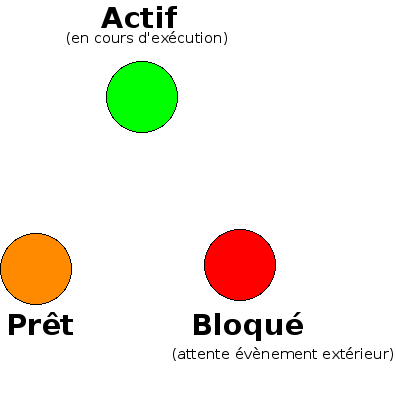
\includegraphics[width=0.7\linewidth]{Figures/actif-pret-bloque.png}
\end{center}



\subsection{Changements d'état}
\begin{enumerate}
\item
Quand le processus actif a besoin de faire une opération
d'entrée-sortie (E/S), il en fait la demande auprès du système
d'exploitation par un ``appel système'' (sous Unix : \texttt{read},
\texttt{write}, etc.).

Si il faut attendre la fin de cette opération pour continuer (par
exemple pour une lecture), le système change l'état du processus, qui
devient \textbf{bloqué}. On parle d'opération \emph{bloquante}.

  \begin{center}
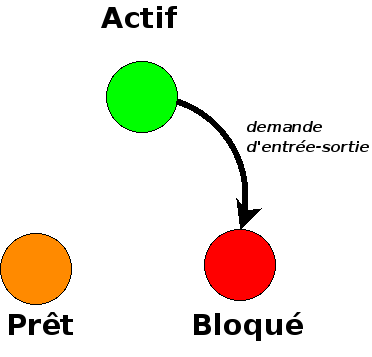
\includegraphics[width=0.7\linewidth]{Figures/actif-vers-bloque.png}
  \end{center}
\item lorsqu'un périphérique signale au processeur qu'une opération d'E/S est achevée, 
le système d'exploitation ``débloque'' le processus qui attendait la fin de cette opération.
Le processus est alors marqué comme \textbf{prêt}.

  \begin{center}
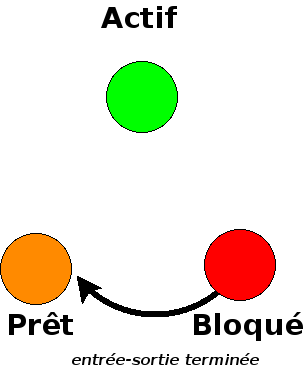
\includegraphics[width=0.7\linewidth]{Figures/bloque-vers-pret.png}
  \end{center}

\item enfin, le système d'exploitation peut choisir un processus prêt 
pour le rendre \textbf{actif}. 
\begin{center}
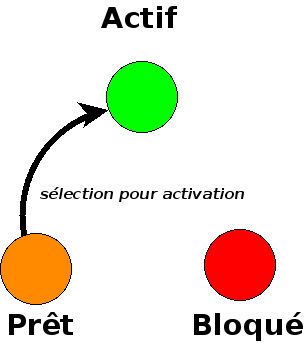
\includegraphics[width=0.7\linewidth]{Figures/pret-vers-actif.png}
\end{center}

Ce changement peut se faire quand le processus actif se termine ou se bloque, 
et ``laisse sa place''.

À un moment donné il peut y avoir plusieurs processus prêts : le choix du processus
à activer est fait par un module appelé  \textbf{ordonnanceur} (\textbf{scheduler}).
Diverses \textbf{politiques d'ordonnancement} sont envisageables, nous les verrons en 
détail plus loin.

\end{enumerate}


\subsection{Multitâche coopératif}

Dans un système multi-tâches dit ``coopératif'', les changements d'états
d'un processus se font donc selon le cycle suivant, qui résume les transitions
vues plus haut :

\begin{center}
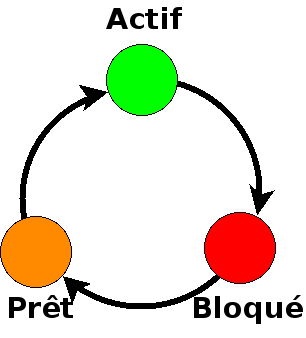
\includegraphics[width=0.7\linewidth]{Figures/pret-actif-bloque2.png}
\end{center}

On observe que le processus qui est actif le reste tant
qu'il ne demande pas d'opérations d'entrée-sortie.

Dans un tel système, Il est donc nécessaire que les programmes soient bien écrits pour 
\begin{itemize}
\item ne pas boucler  indéfiniment
\item faire des entrées-sorties de temps en temps pour ``bien se comporter'' envers les autres processus et leur laisser des occasions de
  s'activer.
\end{itemize}

Évidemment ce genre de système marche assez mal en pratique. C'est ce
qu'on trouvait dans Windows jusqu'à la version 3.11, et Mac OS
jusqu'à MAC OS 9, plus de trente ans après l'invention du ``vrai''
multitâche !

\subsection{Scénario détaillé}

Le schéma ci-dessous montre le déroulement détaillé d'une opération  d'entrée-sortie.
On suppose qu'il y a au départ un processus A qui demande une lecture sur un
périphérique inoccupé, et un processus B qui est prêt.

La scénario montre de haut en bas les ``lignes de vie'' des différentes activités : 
une pour le périphérique, et trois pour le processeur, pour distinguer ce qui relève du système, et des 2 processus.

Les flèches horizontales montrent les causalités.

\begin{center}
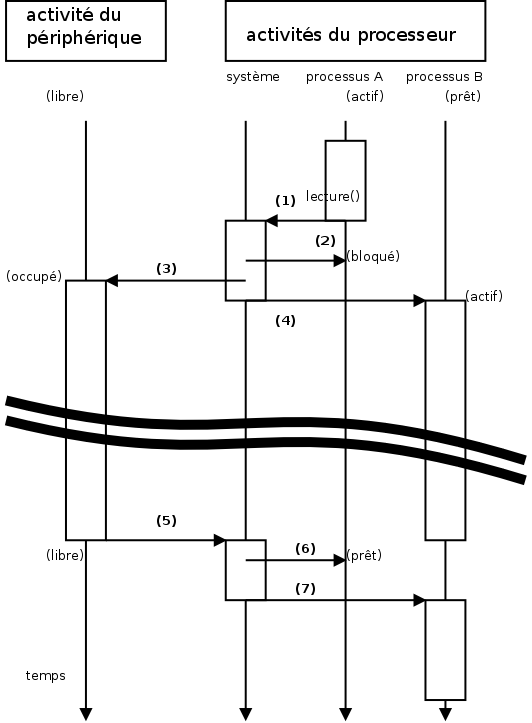
\includegraphics[width=\linewidth]{Figures/deroulement-es.png}
\end{center}

\begin{enumerate}
\item A fait un appel au système d'exploitation pour demander une
  lecture.
\item le système marque le processus A comme bloqué
\item il ordonne au périphérique de se mettre au travail
\item il active B
% \item B s'exécute
\item le périphérique signale la fin de l'opération
\item l'interruption rend la main au système d'exploitation,
qui marque A comme prêt
\item le système rend la main au processus B
\end{enumerate}


\subsection{Multitâche préemptif}

Le multi-tâches préemptif, qui traite correctement les problèmes de
partage du temps, a été proposé très tôt par McCarthy et Teager. Dans
un papier de 1959, McCarty écrit que ``l'idée n'est pas vraiment
nouvelle''.

En fait, il suffit d'ajouter un circuit d'horloge qui envoie une
interruption au bout d'un certain délai.  Quand le système active un
processus, il programme cette horloge pour un certain \textbf{quantum
  de temps}. Il peut alors se passer deux choses
\begin{itemize}
\item soit le processus actif fait un appel système pour faire une E/S
  ou se terminer, et donc il ``passe la main'', au moins
  provisoirement, au système d'exploitation.
\item soit il fait uniquement du calcul, et se trouve donc interrompu,
  automatiquement, par le signal d'horloge quand le quantum de temps
  est épuisé. Le processus est alors marqué comme \texttt{prêt}.
\end{itemize}


    \begin{center}
      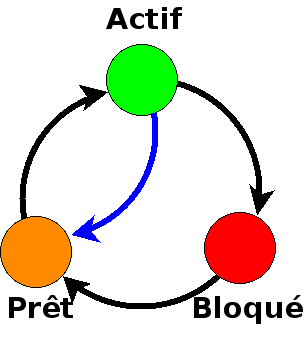
\includegraphics[width=0.7\linewidth]{Figures/pret-actif-bloque3.png}
    \end{center}

C'est ce qu'on appelle une \textbf{préemption}, capacité pour le système 
d'exploitation d'interrompre une tâche en cours pour activer une tâche plus prioritaire.
 Notez que ceci n'interdit pas que le processus ainsi préempté soit aussitôt
réactivé, si l'ordonnanceur détermine qu'il est le plus prioritaire.


Vu autrement, voici le déroulement d'une préemption, à partir du moment
où l'ordonnanceur a déterminé qu'il fallait activer le processus A :
\begin{center}
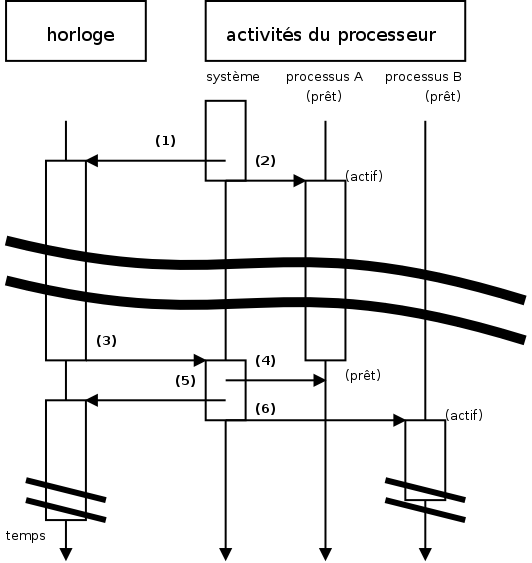
\includegraphics[width=\linewidth]{Figures/deroulement-preemption.png}
\end{center}


\begin{enumerate}
\item le circuit d'horloge est armé pour
un quantum de temps fixé
\item le processus A est activé, et se met à faire du calcul ``indéfiniment''
\item le quantum est épuisé, l'horloge envoie une interruption
\item le système reprend la main
\item le processus A est marqué ``prêt''
\item le processus B est choisi et activé, l'horloge est armée.
\end{enumerate}

Dans ce système dit ``multi-tâches préemptif'' on a donc la garantie que
le système d'exploitation reprend la main régulièrement, ce qui lui
donnera l'occasion de distribuer le temps équitablement entre les
processus non-bloqués, sans laisser un processus actif monopoliser le
processeur.


Le multitâche préemptif est présent sur tous les
ordinateurs multitâches depuis les années 60.  On mesure donc à quel point, 
pendant la décennie 1980-1990, les principaux systèmes pour micro-ordinateurs (Windows et MacOS)
étaient littéralement préhistoriques.


En effet, ces petits systèmes ont revécu, trente ans plus tard, l'histoire de l'informatique :
\begin{itemize}
\item au départ, petites machines à capacité très limitées
\item utilisées par un seul programme à la fois, une seule personne à
  la fois. Dans le cas de la micro-informatique, l'objectif commercial était de vendre un ordinateur par
  personne, surtout pas de le partager à plusieurs !
\end{itemize}
L'évolution vers le multi-tâche a été forcée par l'utilisation
d'interfaces graphiques (si on a un multi-fenêtrage, on veut fatalement  y faire
tourner plusieurs programmes). Le multi-tâche coopératif est assez
facile à réaliser par modification d'un système mono-tâche. Par contre
le passage au multitâche préemptif nécessitait une refonte complète du
système, ainsi que du catalogue d'applications.\footnote{On le sait
  assez peu, mais la société Microsoft prévoyait, après le lancement
  de DOS 3.0, de faire évoluer son catalogue vers Xenix, un système
  UNIX dont elle avait acheté les droits à ATT à la fin des années 70
  de façon à pouvoir enfin remplacer DOS par un vrai système
  multitâches. Ce plan a été abandonné vers 1985, quand Microsoft et
  IBM ont commencé à développer ensemble OS/2 (nom de code ``CP/DOS'')
  qui devait préserver la compatibilité avec les applications
  existantes. En effet, commercialement, il est mal avisé de forcer
  les clients à racheter tout leur parc logiciel pour bénéficier d'un
  nouveau système, fut-il techniquement bien meilleur. La stratégie OS/2 a
  aussi été abandonnée au profit du développement de 
  Windows NT, qui regroupe en fait
  les versions Windows 2000, XP, 2003, Vista, Home Server, Server
  2008, et Windows 7.  }



\subsection{Multitâche préemptif et utilisation interactive}

Soient deux utilisateurs X et Y d'un ordinateur en temps-partagé. Ils
lancent tous les deux, à peu près en même temps, un programme qui fait une minute de calcul.

\begin{itemize}
\item 
Dans le cas d'un système coopératif, le calcul de l'un sera effectué pendant une minute,
et alors commencera le calcul du second.
\item
Dans un système préemptif, les deux calculs alterneront par petites tranches correspondant au quantum de temps
(valeurs courantes entre 1/50 et 1/1000 de seconde).  Ils finiront donc tous les deux au bout de deux minutes.
\end{itemize}

En résumé, dans le cas coopératif, l'attente moyenne des deux utilisateurs sera 
$\frac{60+120}{2} = 90 s$, et avec le système coopératif 
$\frac{120+120}{2} = 120 s$.

\begin{exercice}
L'attente moyenne est-elle un bon critère pour mesurer la satisfaction
des utilisateurs d'un système en temps partagé ?  Pouvez-vous proposer
mieux ?
\end{exercice}


\subsection{Interruptions et multitâche, en résumé}

Une interruption est un signal qui détourne le processeur de sa boucle
  d'exécution normale (lire une instruction, l'exécuter, passer à la
  suivante), pour effectuer un traitement particulier (routine de
  traitement d'interruption).

Les interruptions sont causées par
\begin{itemize}
  \item les \textbf{périphériques} (fin d'exécution de requête)
  \item des \textbf{signaux d'horloge}
  \item des \textbf{évènements extérieurs}
  \item déroutements en cas d'\textbf{erreur} (accès illégal à la mémoire,
  division par zéro ...)
  \item \textbf{interruptions logicielles} provoquées par instruction spéciale 
\end{itemize}

Dans un système d'exploitation multitâches, les interruptions sont traitées par le système, qui 
agit sur l'état des processus :

\begin{itemize}
\item venant d'un périphérique d'E/S : le système fait passer le
  processus demandeur à l'état prêt ;
\item venant de l'horloge (épuisement du quantum de temps), le système
  fait passer le processus actif à l'état prêt;
\item interruption d'erreur (division par zéro etc) : le processus
  actif est supprimé.
\end{itemize}



\section{Politiques d'ordonnancement}

\subsection{Ordonnanceur}

Dans un système d'exploitation multi-tâches, l'\textbf{ordonnanceur} (\emph{scheduler})
est un composant du noyau, qui a pour fonction de choisir un des processus prêts pour l'activer.

L'ordonnanceur applique une \textbf{politique d'ordonnancement}, algorithme ou heuristique qui est censé donner ``de bons résultats''.

\subsection{Critères d'évaluation}

Une politique d'ordonnancement peut être évoluée selon plusieurs critères. On peut en effet souhaiter avoir
\begin{itemize}
\item \textbf{équité}  : chaque processus dispose d'une part équitable 
du temps global, 
\item \textbf{aucun n'est empêché de tourner} (par exemple par une coalition de processus
prioritaires)
\item \textbf{minimiser le temps de réponse}  : les utilisateurs interactifs souhaitent un système ``réactif''. Quand ils lancent des commandes courtes, la réponse doit être rapide.
\item \textbf{minimiser le temps d'exécution} : les commandes longues ne s'éternisent pas.
\item \textbf{maximiser le rendement} : on peut lancer davantage de travaux dans la journée.
\end{itemize}

Mais malheureusement
\begin{itemize}
\item ces objectifs sont contradictoires,
\item le comportement des processus ne peut pas être prévu
\end{itemize}.

Il n'y a donc \textbf{pas de politique optimale} valable dans tous les cas.
On se contente d'\textbf{heuristiques}, dont l'expérience montre qu'elles fonctionnent bien
(ou pas) dans des contextes voisins. 

Qui plus est, pour chaque méthode il sera souvent possible de
construire un ``scénario pathologique'' pour lequel les choses se
passent mal, du point de vue d'un critère particulier.  La difficulté est
d'évaluer la probabilité avec laquelle de tels cas peuvent se
produire, dans le contexte d'utilisation visé, ainsi que les
conséquences.

Que des programmes d'affichage puissent
``lagger'' quelques secondes de temps en temps n'a pas la même
importance pour une animation en flash dans un navigateur, et  sur une console
d'aiguilleur du ciel.

\subsection{Tourniquet}

L'algorithme du \textbf{tourniquet} (synonymes : \emph{round robbin},
FIFO, premier arrivé-premier servi, ...)

\paragraph{Principe :}
\begin{itemize}
   \item le système détient une liste des processus prêts ;
  \item on choisit, pour l'activer, le premier processus de la liste ;
\item à la fin de son quantum de temps, un processus actif est placé
en fin de liste
\end{itemize}

\paragraph{Propriétés} :  cette heuristique garantit une \textbf{équité} entre les processus, qui ont tous une occasion de tourner.

\begin{exercice}
Soit trois  processus A, B et C à comportements périodiques : ils font du calcul, une opération d'E/S et recommencent (un très grand nombre de fois).
\begin{itemize}
 \item
  Pour A le calcul dure 10  ms, 10 ms pour B, et 45 ms pour C
\item
   une opération d'E/S de 20 ms
\end{itemize}

Étudiez le déroulement pendant les 150 premières ms
\begin{itemize} 
\item pour un ordonnancement circulaire (tourniquet) sans réquisition
\item pour un ordonnancement avec réquisition (quantum 20 ms)
 \end{itemize}

Comparez les taux d'utilisation des CPU dans les deux cas.
\end{exercice}

\subsection{Priorités}

Les priorités permettent de favoriser certains travaux.

On affecte un niveau de priorité (numérique) à chaque processus. Sous
Unix, ce sont les numéros faibles qui sont les plus prioritaires.

\paragraph{Principe}

\begin{itemize}
\item on choisit le processus de priorité la plus élevée
\item si il y a plusieurs processus du même niveau, ils sont sélectionnés à tour de rôle (tourniquet)
\end{itemize}

\paragraph{Propriétés}
\begin{itemize}
\item il y a un risque de \textbf{coalition} : si il y a beaucoup de processus
prioritaires qui font du calcul, ils occupent le temps du processus à eux seuls,
empêchant les autres processus de tourner.
\end{itemize}

\begin{exercice}
Soient deux processus A, B au fonctionnement cyclique : ils font
 du calcul (durées $d_a$, $d_b$), une entrée-sortie (durée $d_{es}$),
 et recommencent.
Un processus C, moins prioritaire, ne fait que du calcul.

À quelle condition apparaît-il une coalition entre A et B qui empêche C de s'exécuter ?
\end{exercice}

\begin{exercice}
   Soient trois processus A, B et C, qui ont un comportement répétitif : ils font un peu de calcul
pour une durée t (respectivement 10ms, 15ms et 45ms), puis une opération d'entrée-sortie (qui
dure 20ms), et recommencent. Le processeur d'entrées-sorties traite les requêtes séquentiellement,
dans l'ordre où il les reçoit.
\begin{enumerate}
\item En supposant un ordonnancement par tourniquet sans réquisition,
  évaluez le taux d'occupation de la CPU, et du processeur
  d'entrées-sorties. Étudiez l'équité de l'ordonnancement.
\item 
  Même question, avec un ordonnancement préemptif avec tourniquet, et
  un quantum fixé à 20 ms.
\item Même question, avec un ordonnancement préemptif avec priorités
  (dans l'ordre décroissant B, A, C), et un quantum fixé à 20 ms.
\end{enumerate}
\end{exercice}

\subsection{Priorités variables}
En pratique on utilise des systèmes avec des priorités variables.

Exemple d'un tel système :
\begin{itemize}
\item chaque processus se voit accorder une priorité initiale (qui peut dépendre de l'utilisateur)
\item la priorité baisse chaque fois que le processus termine son quantum de temps 
\item elle revient à son niveau initial après chaque entrée-sortie.
\end{itemize}

Ainsi
\begin{itemize}
\item les processus qui font beaucoup de calcul sont pénalisés, leur priorité
baisse.
\item les processus courts sont favorisés, ce qui donne 
aux utilisateurs interactifs une impression de réactivité.
\item de même les processus qui font beaucoup d'E/S (et donc chargent
  peu le processeur), ont davantage d'occasions de tourner.
\end{itemize}

\begin{exercice}
Au département informatique nous avons eu un problème avec un système
d'exploitation (SysVr4) qui remontait les priorités les processus qui
faisaient des entrées-sorties.

Les étudiants devaient écrire du code pour afficher les requêtes d'une base
de données, avec un algorithme du style
\begin{lstlisting}
  requete <=  "select * from voitures"
  curseur <=  lancer-requete(req) 

  tant que code-erreur() == 100
    faire 
           afficher valeur(curseur)
           avancer(curseur)
\end{lstlisting}
Dans ce code, les opérations sur la base de données 
communiquent par l'intermédiaire d'un ``\emph{pipe}'' avec
 un processus qui accède effectivement aux fichiers de la base.

Certains étudiants ont inversé le test d'arrêt. Leur programme entrait
donc dans une boucle de conversation avec l'autre processus, qui
répondait immédiatement avec un code d'erreur différent de 100.

Quelles sont les conséquences pour les autres utilisateurs ?
\end{exercice}

\subsection{Files multiples}


On définit des \textbf{classes} de processus
\begin{itemize}
\item à chaque classe correspond une liste (FIFO) de processus
\item chaque classe est sélectionnée régulièrement
\end{itemize}

On décidera par exemple d'avoir 3 classes : A (prioritaire), B
(normal), C (non prioritaire), à qui on accordera respectivement 50
\%, 30 \% et 20 \% du temps de calcul. Chaque classe sera gérée
selon le principe du tourniquet,

Par exemple, pour les 5 premières activations l'ordonnanceur choisira
un processus prêt de la classe A, pour les 3 suivantes dans la classe
B, etc, et recommencera.

Ce système a l'avantage
\begin{itemize}
\item de respecter les priorités,
\item d'interdire les coalitions.
\end{itemize}

Dans l'exploitation en traitement par lots, les classes permettaient
une segmentation de la clientèle des centres de calculs : les tarifs
étaient plus élevés pour les travaux dans la classe la plus
prioritaires. Les clients ``en classe économique'' devaient attendre
les résultats plus longtemps.


\end{multicols}


